\section{Diagnostic Evidence: Prediction, Simple Paths, and Natural State}
\label{sec:early}
\subsection{Prediction closure does not select a useful intervention}
The early studies distinguish prediction/native agreement from reference agreement. B570 changes target prefill UB1-to-UB128 with the prescribed first-pending sample and state handoff; continuation and draft remain UB1. On an exposed 24-task cohort, baseline and intervention predictions each match all 72 repeated native arrays. Reference agreement rises from 60/72 to 72/72: four known deviations recover without a new deviation among 20 controls.

This does not isolate KV alone. Transferred state includes pending logits, positions, and a post-accept sampler clone. The result concerns the recorded intervention, not arbitrary prefill-only repair or performance benefit.

RTX changes target continuation UB2-to-UB1 while retaining recorded prefill, draft, and caller grouping. Predictions reproduce both native conditions on 19 exposed HumanEval tasks and 24 statically selected MBPP tasks: 57 and 72 repeated arrays per condition. Yet HumanEval/15 repairs, /25 regresses, and /18 stays divergent. HumanEval reference agreement remains 51/57, or 17/19 tasks. MBPP remains 66/72, with two persistent failures. An unchanged aggregate hides opposing effects.

One persistent failure also changes its complete output. MBPP/304 retains 47 IDs but changes 488 to 481 at zero-based position 33 while staying divergent. Reference failure, output change, and no-op are distinct. These results motivate controlling execution state and phase; they do not validate the predictor as a repair selector.

\subsection{The ordinary target-only bridge}
A fresh comparison tests whether ordinary draft-free $U_2$ reproduces the RTX intervention $N_1$. It uses the same 19 exposed HumanEval tasks, three conditions, and three fresh-process repetitions: 171 formal runs. Relevant numerical threads are matched at 24; condition order rotates, and no process or KV state is reused. $U_2$ uses its own prefill and continuation, without draft, transplant, proposal tape, or reference answer.

$U_2=N_1$ on all 57 complete arrays and strict stop boundaries. $U_2=N_0$ and $N_0=N_1$ each hold for 51/57 arrays. The changed tasks are the repair and regression above; the other 17 are output no-ops. Each condition is repeat-stable on all 19 tasks, while all retain 17/19 reference agreement.

The simpler path reproduces both nontrivial changes on this cohort. Allocated UB2 does not require two occupied continuation tokens: $U_2$'s observed continuation batches contain one token. Live $U_2$ graph tensors and KV/logits are unavailable, so output equality is not a state-equivalence theorem. The complex predictor is unnecessary for this particular reproduction objective; no timing or general predictive advantage follows.

\subsection{A bounded negative selection result}
An existing-record analysis tests whether paid proxy screening adds a supported configuration-selection capability. A proposed state-fingerprint rule lacks aligned state and a repair direction for implementation. A charged proxy-and-verification replay compares available outcomes with direct enumeration, without exposing unqueried labels.

On RTX19, enumeration and proxy screening both abstain and use 114 post-common-acquisition record equivalents. On B57024, direct verification selects the sole candidate with 72 records; proxy screening selects it with 144. These are retrospective acquisition equivalents, not latency or new inference. MBPP target-only counterfactuals are unavailable and remain unknown.

For a sole accepted action, screening adds proxy/setup work unless it supplies an otherwise unavailable capability or rejection saving. No matched timing establishes that benefit here. Diagnostic fidelity, repair utility, and operational value therefore need separate evidence before retaining additional machinery.


\subsection{Natural state and current execution}

\label{sec:cross}
\subsubsection{RTX: path effects and local interactions}
Four previously exposed HumanEval probes use naturally reached donor states at equal committed prefixes. Across repetitions, 24 donors generate 48 state/current-path forks with 24 own-path shams. Auxiliary probe forwards are separately charged and are not speed measurements. Restoring and continuing an own-path state checks that the manipulation itself reproduces the native decision.

At HumanEval/15, the final verification/bonus decision changes with the current UB2 versus UB1 call under both donors. At HumanEval/25, only the combination of the N1 donor and current UB1 call changes the sampled decision. The latter is an interaction, not a state-only explanation. At the chosen boundaries of /18 and /31, neither intervention changes the discrete decision. A null at these boundaries does not prove trajectory-wide invariance.

\begin{figure}[t]
\centering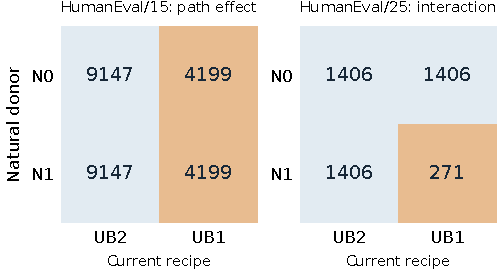
\includegraphics[width=0.62\linewidth]{figures/state_path_cross.pdf}
\caption{RTX natural-state crosses at fixed committed prefixes. /15 shows a current-path effect under both donors; /25 changes only for N1 with UB1. Cells display the discriminating sampled token ID: the third decision for /15 and the first for /25. Colors group equal IDs within each task. These selected cells are local causal observations.}
\label{fig:statepath}
\end{figure}

The donors' prompt K/V tensors agree in all 12 compared pairs, while 70 of 72 generated-prefix tensor comparisons differ. First-layer logical K/V remain equal in the tested pairs.  

The expanded width study supplies another case. MBPP/229 at a natural 47-token prefix fails at wide UB6 verification. Real donor-state crosses under two current query layouts flip EOG argmax with the state; current layout changes continuous scores without independently flipping argmax in the measured cells. Four shams reproduce their own decisions. Two cap contexts are two observations of one task, not two independent counterexamples. This case connects a numerical-state boundary to a wider qualified-execution search without claiming a uniquely causal CUDA kernel.

\subsubsection{B570: a different recipe and the same questions}
On B570, six natural-state crosses with 12 own-path shams cover three tasks in repeated contexts. Byte-validated round trips and KV ownership checks support genuine donor-state manipulation. HumanEval/145 and /42 show local state--whole-recipe interactions. MBPP/72 shows a donor-state effect while its two current-recipe columns are identical controls. It cannot count as an independently varied current-path effect.

Table~\ref{tab:cross} shows representative raw argmax IDs, whose numeric magnitudes have no metric interpretation. The current B570 recipes change microbatch and output-reservation behavior together. The matrix therefore does not isolate one operator. Subsequent counterfactual complete continuations are not available for these cross cells; endpoint recovery is demonstrated separately by native full requests.

\begin{table}[t]
\centering\footnotesize\setlength{\tabcolsep}{3pt}
\caption{Representative B570 $2\times2$ argmax matrices. Rows are natural donor states; columns are the recorded current recipes. /72 has duplicate columns. Cases are local evidence, not prevalence estimates.}
\label{tab:cross}
\begin{tabular}{lcc}\toprule
Task & Donor 0: $(e_0,e_1)$ & Donor 1: $(e_0,e_1)$\\\midrule
HumanEval/145 & $(71465,279)$ & $(279,279)$\\
HumanEval/42 & $(432,1817)$ & $(1817,1817)$\\
MBPP/72 & $(320,320)$ & $(308,308)$\\\bottomrule
\end{tabular}
\end{table}

Together the two GPUs support the portability of the \emph{experimental question}: equal prefixes do not remove the need to control retained state and the current recipe. They do not demonstrate that one constraint, matrix pattern, or parameter choice transfers unchanged between CUDA and Vulkan.

